\documentclass[
  bibliography=totoc,     % Literatur im Inhaltsverzeichnis
  captions=tableheading,  % Tabellenüberschriften
  titlepage=firstiscover, % Titelseite ist Deckblatt
]{scrartcl} % Alternative: scrreprt und scrbook

% Paket float verbessern
\usepackage{scrhack}

% Warnung, falls nochmal kompiliert werden muss
\usepackage[aux]{rerunfilecheck}

% unverzichtbare Mathe-Befehle
\usepackage{amsmath}
% viele Mathe-Symbole
\usepackage{amssymb}
% Erweiterungen für amsmath
\usepackage{mathtools}
\usepackage{dsfont}
% Fonteinstellungen
\usepackage{fontspec}
% Latin Modern Fonts werden automatisch geladen
% Alternativ:
%\setromanfont{Libertinus Serif}
%\setsansfont{Libertinus Sans}
%\setmonofont{Libertinus Mono}

% Wenn man andere Schriftarten gesetzt hat, sollte man
% das Seiten-Layout neu berechnen lassen
\recalctypearea

% Rändermaße
\usepackage[
    left=3cm,
    right=3cm,
    top=1.5cm,
    bottom=2cm,
    includeheadfoot
]{geometry}

% deutsche Spracheinstellungen
\usepackage{polyglossia}
\setmainlanguage{german}


\usepackage[
  math-style=ISO,    % ┐
  bold-style=ISO,    % │
  sans-style=italic, % │ ISO-Standard folgen
  nabla=upright,     % │
  partial=upright,   % ┘
  warnings-off={           % ┐
    mathtools-colon,       % │ unnötige Warnungen ausschalten
    mathtools-overbracket, % │
  },                       % ┘
]{unicode-math}

% traditionelle Fonts für Mathematik
\setmathfont{Latin Modern Math}
% Alternativ:
%\setmathfont{Libertinus Math}

\setmathfont{XITS Math}[range={scr, bfscr}]
\setmathfont{XITS Math}[range={cal, bfcal}, StylisticSet=1]

% Zahlen und Einheiten
\usepackage[
  locale=DE,                   % deutsche Einstellungen
  separate-uncertainty=true,   % immer Fehler mit \pm
  per-mode=symbol-or-fraction, % / in inline math, fraction in display math
]{siunitx}

% chemische Formeln
\usepackage[
  version=4,
  math-greek=default, % ┐ mit unicode-math zusammenarbeiten
  text-greek=default, % ┘
]{mhchem}

% richtige Anführungszeichen
\usepackage[autostyle]{csquotes}

% schöne Brüche im Text
\usepackage{xfrac}

% Standardplatzierung für Floats einstellen
\usepackage{float}
\floatplacement{figure}{htbp}
\floatplacement{table}{htbp}

% Floats innerhalb einer Section halten
\usepackage[
  section, % Floats innerhalb der Section halten
  below,   % unterhalb der Section aber auf der selben Seite ist ok
]{placeins}

% Seite drehen für breite Tabellen: landscape Umgebung
\usepackage{pdflscape}

% Captions schöner machen.
\usepackage[
  labelfont=bf,        % Tabelle x: Abbildung y: ist jetzt fett
  font=small,          % Schrift etwas kleiner als Dokument
  width=0.9\textwidth, % maximale Breite einer Caption schmaler
]{caption}
% subfigure, subtable, subref
\usepackage{subcaption}

% Grafiken können eingebunden werden
\usepackage{graphicx}
% In folgenden Ordnern wird nach den Graphiken gesucht
\graphicspath{
  {images/}{../images/}
  {pics/}{../pics}
  {content/}{../content/}
  {build/}{../build/}
  {rohdaten/}{../rohdaten/}
  {python/}{../python}
}

% größere Variation von Dateinamen möglich
\usepackage{grffile}
% verhindert das Bilder in anderen Sections auftrerten
\usepackage{placeins}

% schöne Tabellen
\usepackage{booktabs}

% Verbesserungen am Schriftbild
\usepackage{microtype}

% Literaturverzeichnis
\usepackage[
  backend=biber,
]{biblatex}
% Quellendatenbank
\addbibresource{src.bib}
\addbibresource{programme.bib}

% Hyperlinks im Dokument
\usepackage[
  unicode,        % Unicode in PDF-Attributen erlauben
  pdfusetitle,    % Titel, Autoren und Datum als PDF-Attribute
  pdfcreator={},  % ┐ PDF-Attribute säubern
  pdfproducer={}, % ┘
]{hyperref}
% erweiterte Bookmarks im PDF
\usepackage{bookmark}

% Trennung von Wörtern mit Strichen
\usepackage[shortcuts]{extdash}

\author{
  Patrick Schmidt
  \texorpdfstring{
    \\
    \href{mailto:patrick7.schmidt@udo.edu}{patrick7.schmidt@udo.edu}
  }{}
  \texorpdfstring{\and}{, }
  Karl Schiller
  \texorpdfstring{
    \\
    \href{mailto:karl.schiller@udo.edu}{karl.schiller@udo.edu}
  }{}
}

% keine Lücke am Beginn eines Absatzes lassen
\setlength{\parindent}{0pt}
% Zwischen den Absätzen eine Leerzeile einbauen
\setlength{\parskip}{\baselineskip}

% Füllwort bei SIrange verändern
\sisetup{mode=text,range-phrase={\text{ bis }}}
% Neue Buchstaben bei SIunitx
\sisetup{math-micro=\text{µ},text-micro=µ}

% Bilder von Text umfließen lassen
\usepackage{wrapfig}

% Ermögliche Befehl \mean für einen Mittelwert
\newcommand*\mean[1]{\bar{#1}}

%% EOF %%


\subject{VERSUCH NUMMER 48}
\title{Dipolrelaxation in Ionenkristallen}
\date{
  Durchführung: 03.06.2019
  \hspace{3em}
  Abgabe: 07.06.2019 \\
  \vspace{0.5cm}
  1. Korrektur: 11.06.2019
}
\subtitle{\centering Fakultät Physik \\
Technische Universität Dortmund}
\begin{document}

\thispagestyle{empty}
\maketitle
\thispagestyle{empty}
\tableofcontents
\newpage
\setcounter{page}{1}

\section{Zielsetzung}
\label{sec:Zielsetzung}
Ziel des Versuchs ist es die Aufspaltung der Energieniveaus durch den Zeeman-Effektes,
sowie der Hyperfeinstruktur auszumessen. Des Weiteren soll der Landé-Faktor des Gesamtdrehimpulses
des Atoms bestimmt werden. Ebenso soll das transidente Verhalten näher untersucht werden.

\section{Theorie}
\label{sec:Theorie}
\subsection{Atomaufbau}
\label{sec:atomaufbau}
Aus der Quantenmechanik ist bekannt, dass das Atom aus einem Kern und einer Atomhülle besteht.
In der Atomhülle bewegen sich die Elektronen auf festen Energieniveaus. Dabei sind die inneren
Niveaus voll besetzt. Die äußeren Niveaus sind nach der Boltzmann-Verteilung
\begin{equation}
  \label{eqn:boltz}
  \frac{N_2}{N_1} = \frac{g_2 \cdot \exp{\left(\sfrac{-W_2}{k_\text{B}T}\right)}}{g_1 \cdot \exp{\left(\sfrac{-W_1}{k_\text{B}T}\right)}}
\end{equation}
temperaturabhängig besetzt. Dabei bezeichnen die $N_\text{i}$ die Besetzungszahlen, $g_\text{i}$ den Entartungsgrade
der Energieniveaus $W_\text{i}$, wobei $W_2 > W_1$ gilt. Damit die Formel auch ihre Gültigkeit besitzt
muss sich das Atom bei Temperatur $T$ im thermischen Gleichgewicht befinden.
Um zwischen den Energieniveaus zu wechseln müssen Quanten der Energie
\begin{equation}
  \label{eqn:energiedifferenz}
  h \nu = W_2 - W_1
\end{equation}
emittiert oder absorbiert werden. 
In diesem Versuch werden Alkaliatome untersucht, diese zeichnen sich dadurch aus, dass sich nur ein 
Elektron auf dem äußersten Niveau befindet, was die Rechnungen deutlich vereinfacht.

\subsection{Magnetisches Moment der Atomhülle}
\label{sec:atomhülle}
Aus dem Bahndrehimpuls der Eektronen $\vec{L}$ und dem Spin der Elektronen $\vec{S}$ ergibt sich der
Gesamtdrehimpulses $\vec{J} = \vec{L} + \vec{S}$. Zu jedem Drehimpuls gehört auch ein magnetisches Moment.
Dabei ergibt sich das magnetische Moment für den Gesamtdrehimpuls 
\begin{equation*}
  \vec{\mu_\text{J}} = \vec{\mu_\text{L}} + \vec{\mu_\text{S}}
\end{equation*}
aus der Summe der magnetischen Momente für Spin 
\begin{equation}
\label{eqn:magspin}
  \vec{\mu_\text{S}} = -g_\text{S} \mu_\text{B} \vec{S}
\end{equation}
und Bahndrehimpuls
\begin{equation}
  \label{ean:magbahn}
  \vec{\mu_\text{L}} = - \mu_\text{B} \vec{L}.
\end{equation}
Mit dem Betrag eines jeden Drehimpulses $|\vec{L'}| = \sqrt{L' \left(L'+1\right)}$ und den
in Abbildung \ref{fig:magnmoment} dargestellten Zusammenhängen ergibt sich nach Anwenden des Kosinussatzes
und umstellen
\begin{equation}
  \label{eqn:gj}
  g_\text{J} = \frac{\num{3.0023}J(J+1)+\num{1.0023}[S(S+1)-L(L+1)]}{2J(J+1)},
\end{equation}
dabei wird $g_\text{S} = \num{2.00232}$ verwendet.
Wird nun ein äußeres Magnetfeld $\vec{B}$ angelegt, so spalten sich die Energieniveaus in $2J+1$ Unterniveaus auf.
Dies hat seine Ursache in der Wecheselwirkung des magnetischen Moments mit dem Magnetfeld und der Richtunsquantelung.
Bekanntlich präzidiert $\vec{\mu_\text{J}}$ um die Feldrichtung des äußeren magnetfeldes und der senkrtechte Anteil mittelt 
sich herraus. Für die $z$-Komponete ergibt sich mit der Richtungsquantelung die Wecheselwirkungsenergie zu
\begin{equation}
  \label{eqn:wwenergie}
  U_\text{magn} = M_\text{J} g_\text{J} \mu_\text{B} |\vec{B}|,
\end{equation}
mit der Orientierungsquantenzahl $M_\text{J} = -J, \ldots, J-1 ,J$. Dieser Effekt ist besser bekannt unter
dem Namen Zeeman-Effekt.
\begin{figure}
  \centering
  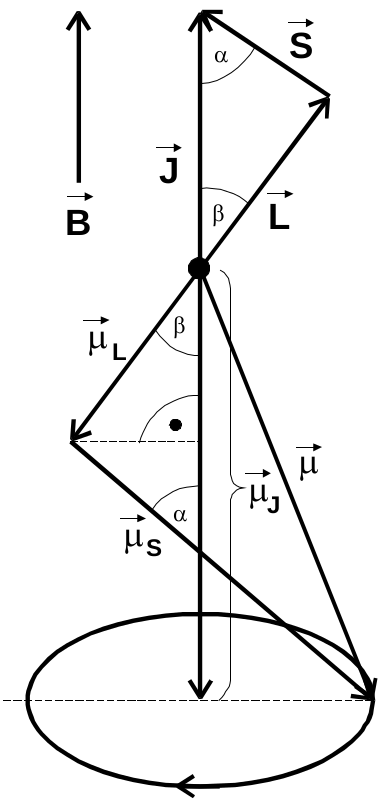
\includegraphics[height=5.5cm]{content/pictures/MagnMoment.png}
  \caption{Skizze zur Veranschaulichung der Zusammenhänge für die Bestimmung des magnetischen Moments der Elektronenhülle \cite{anleitung}.}
  \label{fig:magnmoment}
\end{figure}

\subsection{Magnetisches Moment des Atoms}
\label{sec:atom}
Neben den Hüllenelektronen trägt auch der Kern mit seinem Kernspin $I$ zum Gesamtdrehimpuls des Atoms $F$ bei.
Dabei verläuft dies analog zu Abschnitt \ref{sec:atomhülle}, genauer
\begin{equation*}
  \vec{F} = \vec{J} + \vec{I}.
\end{equation*}
Auf Grund der Kopplung vom Kernspin mit dem Gesamtdrehimpuls der Atomhülle ergibt sich die Aufspaltung der 
Hyperfeinstruktur, dabei darf das äußere Magnetfeld allerdings nicht zu stark sein.
Es ergeben sich $2J+1 (J<I)$ beziehungsweise $2I+1 (I<J)$  Unterniveaus. Dies Unterniveaus werden mit Hilfe
der Quantenzahl $F = |I-J|, \ldots,I+J-1, I+J$ unterschieden. Es spalten sich also zunächst die Feinstrukturniveaus
in die Hyperfeinstrukturniveaus auf, welche unter dem Einfluss eines äußeren Magnetfelds weiter in die 
Zeeman-Niveaus aufspalten. Die Energiedifferenz der Zeeman-Niveaus ergibt sich zu
\begin{equation}
  \label{eqn:zeeman}
  U_\text{Z} = g_\text{F} \mu_\text{B} |\vec{B}|.
\end{equation}
Mit Hilfe des magnetischen Moments des Atoms
\begin{equation*}
  \vec{\mu_\text{F}} = -g_\text{F} \mu_\text{B} \vec{F}
\end{equation*}
und der richtungsorientierten Addition der Beiträge der magnetischen Momente von Atomkern und Atomhülle
ergibt sich der Landé-Faktor
\begin{equation}
  \label{eqn:lande}
  g_\text{F} = g_\text{J} \frac{F(F+1)+J(J+1)-I(I+1)}{2F(F+1)}.
\end{equation}

\subsection{Optisches Pumpen}
\label{sec:pumpen}
Als optisches Pumpen wird eine Umbesetzung der thermischen Besetzung der Energieniveaus bezeichnet.
Um dieses Pumpen zu ermöglichen wird die in Abschnitt \ref{sec:atomhülle} beschriebene Zeeman-Aufspaltung benötigt.
Für ein Alkaliatome ergibt sich im Grundzustand ein $\ce{^2 S_{\sfrac{1}{2}}}$ Niveau, sowie die Niveaus
$\ce{^2 P_{\sfrac{1}{2}}}$ und $\ce{^2 P_{\sfrac{3}{2}}}$ für den ersten angeregten Zustand, wenn der
Kerndrehimpuls vernachlässigt wird. Abbildung \ref{fig:aufspaltung} zeigt die Zeeman-Aufspaltung in die Zeeman-Niveaus für
die beiden Zustände mit $J=\sfrac{1}{2}$, also den optischen $\text{D}_1$-Übergang. Unter zu Hilfe nahme der Auswahlregeln für erlaubte Übergänge
\begin{align*}
  \Delta L & = \pm 1 \\
  \Delta M_\text{J} & = 0, \pm 1
\end{align*}
\begin{figure}
  \centering
  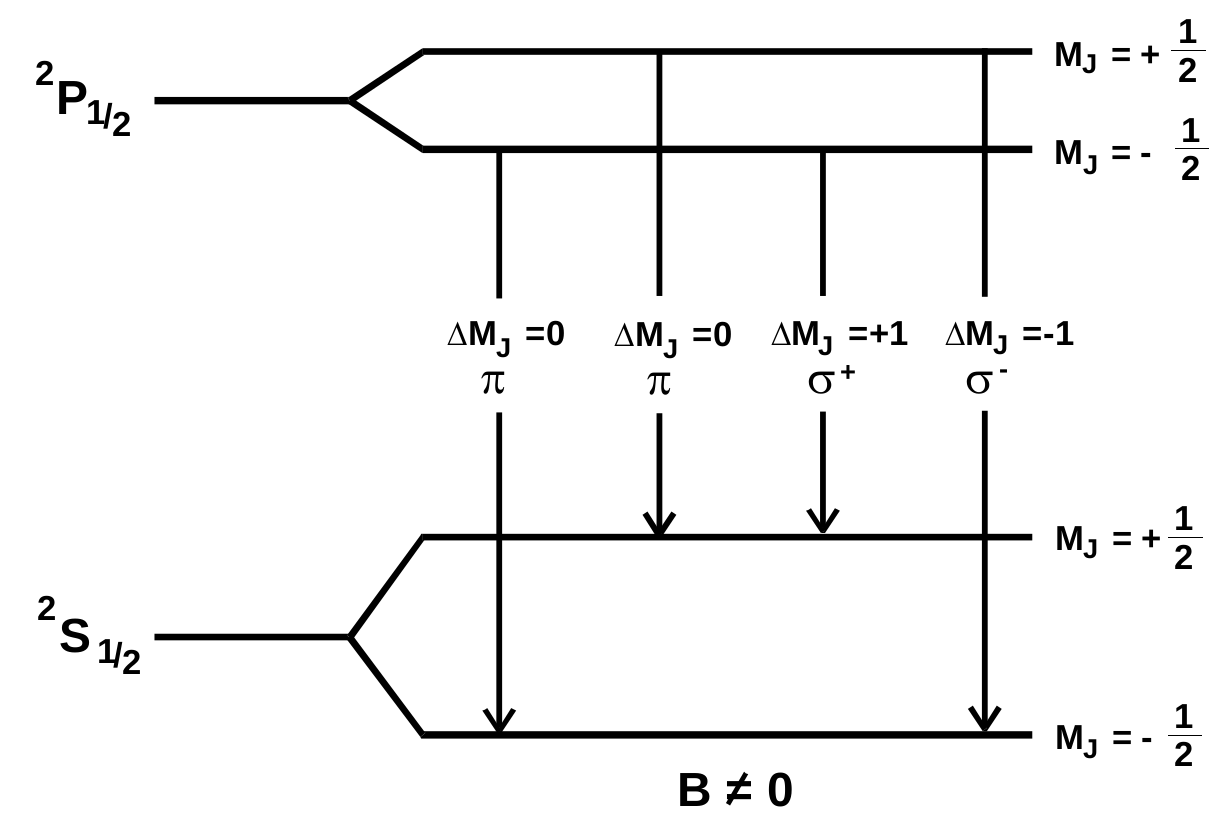
\includegraphics[height=8cm]{content/pictures/Energieniveaus.png}
  \caption{Die Energieniveau-Aufspaltung unter Einfluss eines $\vec{B}$-Feldes \cite{anleitung}.}
  \label{fig:aufspaltung}
\end{figure}
ergeben sich die in Abbildung \ref{fig:aufspaltung} als Pfeile eingezeichneten Übergänge.
Diese unterscheiden sich in Polarisation und Energie der ausgesendeten Quanten. So entspricht 
in Richtung von $\vec{B}$ ausgesendetes rechtszirkular-polarisiertes Licht dem $\sigma^+$-Übergang und 
linkszirkular-polarisiertes Licht dem $\sigma^-$-Übergang. Bei den $\pi$-Übergängen 
handelt es sich um emittiertes beziehungsweise absorbiertes Licht, welches linear-polarisiert
(parallel zu $\vec{B}$) ist und senkrecht zu $\vec{B}$ abgestrahlt wird.

Wird eine Dampfzelle bei der Temperatur $T$ mit einem Dampf aus Alkaliatomen befüllt und 
mit einem Magnetfeld durchsetzt, so befinden sich die Atome zunächst im Grundzustand. Nun wird rechtszirkular-polarisiertes
$\text{D}_1$-Licht eingestrahlt und damit der Übergang mit $\Delta M_\text{J} = +1$ ermöglicht. 
Dadurch werden die Elektronen aus dem $\ce{^2 S_{\sfrac{1}{2}}}$-Niveau mit $M_\text{J}=\sfrac{-1}{2}$ in das 
$\ce{^2 P_{\sfrac{1}{2}}}$-Niveau mit $M_\text{J}=\sfrac{1}{2}$ angehoben. Da es für die Emission
keine weiteren Einschränkungen gibt, finden beide Übergänge ins Grundniveau statt. Es werden aber immer nur
Elektronen aus dem Niveau mit $M_\text{J}=\sfrac{-1}{2}$ angeregt und da kein Übergang innerhalb eines 
Niveaus erlaubt ist, reichern sich die Elektronen im Niveau mit
$M_\text{J}=\sfrac{1}{2}$ an und das mit $M_\text{J}=\sfrac{-1}{2}$ wird entleert. Somit ergibt sich eine 
nicht nach \eqref{eqn:boltz} gegebene thermische Besetzung. 
Mit Hilfe einer Photozelle auf der anderen Seite der Zelle wir die Transparenz des Gases beobachtet.
Wird das $\ce{^2 S_{\sfrac{1}{2}}}$-Niveau ($M_\text{J}=\sfrac{1}{2}$) leer, so wird kein $\text{D}_1$-Licht
mehr absorbiert und die Intensität steigt an. Dieser Verlauf ist exemplarisch in Abbildung \ref{fig:intensität}
dargestellt.
\begin{figure}
  \centering
  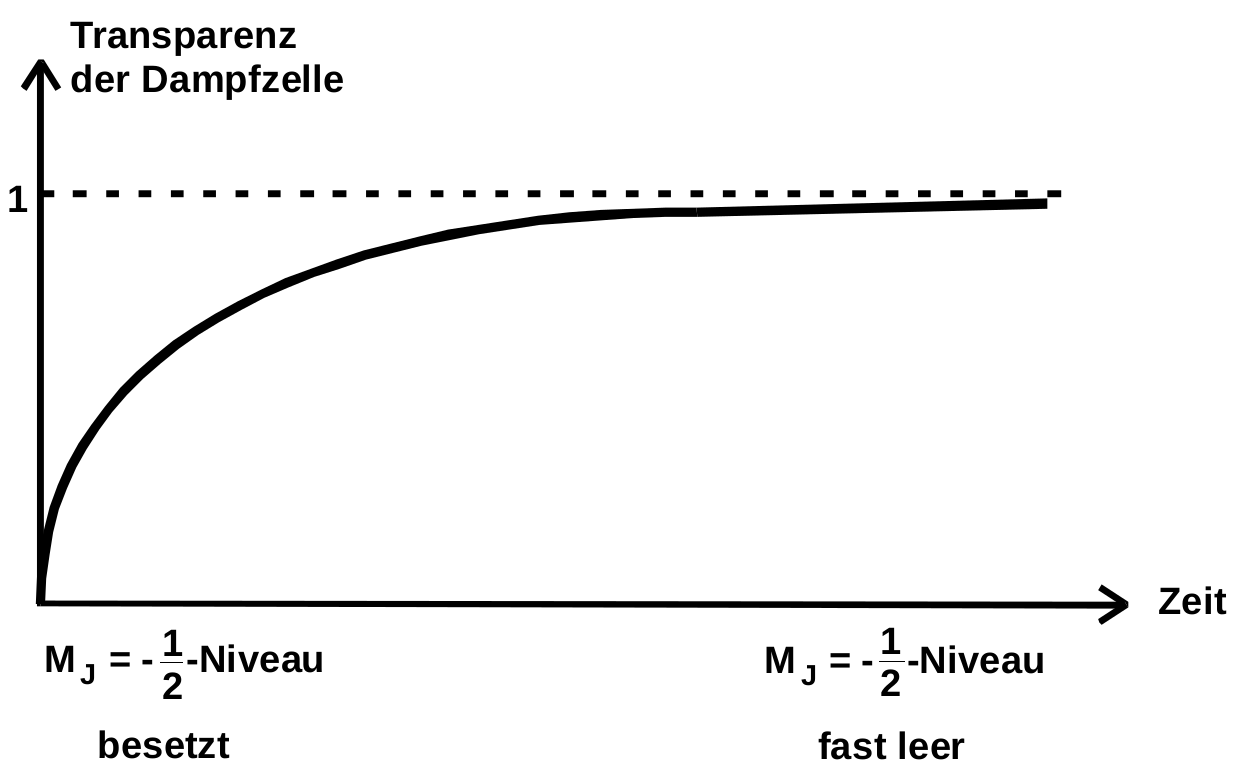
\includegraphics[height=5.5cm]{content/pictures/Transparenz.png}
  \caption{Exemplarischer Verlauf für die Transparenz der Dampfzelle in Abhängigkeit der Zeit \cite{anleitung}.}
  \label{fig:intensität}
\end{figure}

\subsection{Induzierte Emission}
\label{sec:emission}
Wie im vorherigen Abschnitt beschrieben kommt es zur Abregung des angeregten
Niveaus durch Emission von Lichtquanten. Dabei entspricht die Energie der Quanten genau der 
Energiedifferenz der beiden beteiligten Niveaus. Diese Emissionen können nicht nur
spontan auftreten, sondern auch eingeleitet werden, die so genannte induzierte Emission.
Dabei wird ein Lichtquant mit der Energie der Energiedifferenz \eqref{eqn:energiedifferenz} der beiden beteiligten 
Niveaus eingestrahlt, anschließend werden zwei Lichtquanten emittiert. Ob die spontane
oder die induzierte Emission  überwiegt ist rein von der Energiedifferenz des Übergangs abhängig.
Betrachtet man eine große Menge an Gasatomen im Temperaturgleichgewicht der Temperatur $T$, dabei befinden 
sich $N_2$ davon im angeregtem Zustand $W_2$ und $N_1$ im Grundzustand der Energie $W_1$.
Mit der Übergangswahrscheinlichkeit für die spontane Emission $A_{21}$ ergibt sich die Anzahl an 
spontanen Emissionen pro Zeiteinheit zu
\begin{equation*}
  n_\text{spon} = A_{21} N_2.
\end{equation*}
Auf Grund des Temperaturgleichgewichts, steht das Gas im Gleichgewicht mit seiner
Temperaturstrahlung, was der Strahlung eines schwarzen Körpers
\begin{equation*}
  u(\nu) = \frac{8 \pi h \nu^3}{c^2 \cdot \left(\exp{\frac{\nu h}{k_\text{B} T}} -1 \right)}
\end{equation*}
entspricht. Dabei können die Lichtquanten der Frequenz $\nu$, welche genau der Energiedifferenz zweier Niveaus entspricht
eine induzierte Emission auslösen. Dabei ergibt sich die Anzahl der induzierten Emission pro Zeiteinheit zu 
\begin{equation*}
  n_\text{ind} = B_{21} N_2 u(\nu),
\end{equation*}
mit dem Proportionalitätsfaktor der spontanen Emission $B_{21}$, der auch als Einstein-Koeffizient bezeichnet wird.
Es ist aber nicht nur die Abregung dieses Übergangs möglich sondern ebenso die Anregung, also der Übergang
vom Grundzustand in den angereten Zustand. Dabei ergibt sich die Anzahl der von Grundzustand in den angeregten Zustand
übergehenden Elektronen pro Zeiteinheit mit dem Einstein-Koeffizient für die Anregung zu
\begin{equation*}
  n_\text{an} = B_{12} N_1 u(\nu).
\end{equation*}
Da sich das System im thermischen Gleichgewicht befindet, darf sich die Besetzungszahl der Zustände nicht ändern,
es müssen sich also zu jedem Zeitpunkt die nach Formel \eqref{eqn:boltz} gegebenen Besetzungen ergeben. In Formeln ausgedrückt
ergibt sich dann
\begin{equation*}
  n_\text{spon} + n_\text{ind} = n_\text{an}.
\end{equation*}
Für den Fall nicht entarteter Niveaus gilt $B_{21} = B_{12}$, damit ergibt sich
\begin{equation}
  \label{eqn:a}
  A_{21} = \frac{8 \pi h B_{12} \nu^3}{c^3}.
\end{equation}
\begin{figure}
  \centering
  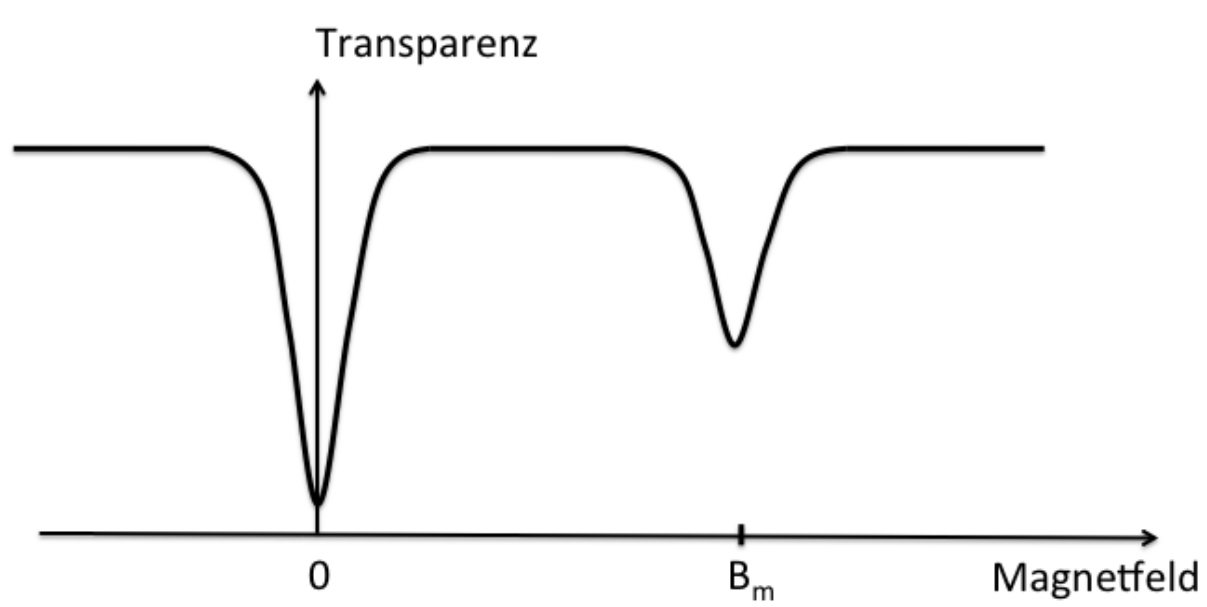
\includegraphics[height=5.5cm]{content/pictures/Resonanz.png}
  \caption{Die Transparenz der Dampfzelle in Abhängigkeit der Zeit für den Fall der Resonaz. \cite{anleitung}.}
  \label{fig:resonanz}
\end{figure}
Der Einstein-Koeffizient kann als Konstante betrachtet werden, da dieser nur von der Gestalt der 
Wellenfunktionen der beteiligten Niveaus abhängt. Da die Energiedifferenz zweier benachbarten Zeeman-Niveaus viel kleiner als
die der Übergänge zwischen Grundzustand und angeregtem Zustand ist, spielt die
spontane Emission also hier keine große Rolle. Bei der Ausmessung der Zeeman-Niveaus tritt also hauptsächlich
induzierte Emission durch die eingestrahlte Hochfrequenzstrahlung auf.
Stellt man also die eingestrahlte Hochfrequenzstrahlung durch das frequenzvariable Hochfrequenzfeld (RF) so ein,
dass genau solch eine Energiedifferenz getroffen wird, kommt es zur Resonanz.
Diese Resonanz tritt also auf, wenn die eingestrahlten Quanten genau der Energie der Zeeman-Aufspaltung nach Formel \eqref{eqn:zeeman} entsprechen.
Also 
\begin{equation*}
  h \nu = g_\text{J} \mu_\text{B} B_\text{m} \Delta M_\text{J}
\end{equation*}
entspricht. Dabei bricht dann die Transparenz der Gaszelle wieder ein, da nun das $\ce{^2 S_{\sfrac{1}{2}}}$-Niveau mit $M_\text{J}=\sfrac{-1}{2}$ wieder 
bevölkert wird. Es ergibt sich der in Abbildung \ref{fig:resonanz} skizzierte Verlauf.
Das Absinken der Transparenz um den Wert $\vec{B}=\vec{0}$ hängt damit zusammen, dass hier keine Aufspaltung in Zeeman-Niveaus vorliegt
und somit kein pumpen möglich ist. In der Realität muss man das Erdmagnetfeld beachten, denn das 
künstlich erzeugte Magnetfeld hat zwar den Wert Null, allerdings erzeugt das Erdmagnetfeld eine Aufspaltung. Die Einstellung der Nullfeld-Linie
stellt also eine gute Möglichkeit dar das Erdmagnetfeld zu bestimmen.

\begin{figure}
  \centering
  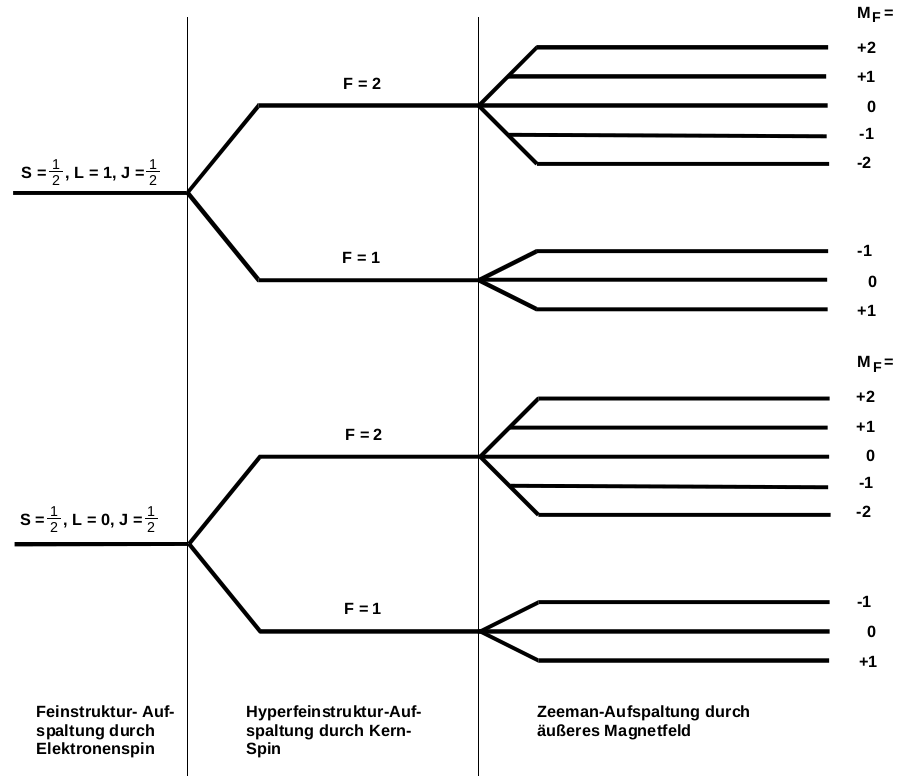
\includegraphics[height=10cm]{content/pictures/Energieniveaus2.png}
  \caption{Die Energieniveau-Aufspaltung unter Einfluss eines $\vec{B}$-Feldes und unter Beachtung des Kernspins \cite{anleitung}.}
  \label{fig:aufspaltung2}
\end{figure}
Wird nur auch der Kernspin beachtet, so ergeben sich leichte Änderungen. Das verwendete Licht wird durch eine Spektrallampe erzeugt und 
auf Grund des Doppler-Effekts ist die Energieverteilung sobreit, dass alle Übergänge der 
Hyperfeinstruktur und der Zeeman-Aufspaltung (siehe hierzu Abbildung \ref{fig:aufspaltung2}) möglich sind und nicht nur der Übergang aus
dem Grundzustand in den ersten angeregten Zustand. Da das Licht rechtszirkular-polarisiert ist
muss $M_\text{F} = +1$ erfüllt werden. Aus eben diesem Grund kann der Zustand $F = 2, M_\text{J} = 2$ keine
eingestrahlten Lichtquanten absorbieren, da kein angeregter Zustand mit $M_\text{F} = 3$ existiert. Die Besetzung dieses Zustands
kann also während des Pumpens nur zunehmen, da er durch die angeregten Zustände mit $M_\text{F} = 2, 1$ bevölkert wird, aber nicht entleer.
Nun kann aber wieder mit Hilfe von Hochfrequenzstrahlung eine induzierte Emission zwischen den Zeeman-Niveaus erzwungen werden.

Wird das äußere Magnetfeld zu stark, so wird ein Teil der inneren Kopplungen aufgehoben und 
es müssen Terme höherer Ordnung beachtet werden. Der sogenannte quadratische Zeeman-Effekt sorgt dabei, dass nicht mehr alle 
Zeeman-Übergänge gleich groß sind. Die Energiedifferenz der Zeeman-Aufspaltung ergibt sich nun nach
\begin{equation}
  \label{eqn:zeemanquadrat}
  U_\text{Z} = g_\text{F} \mu_\text{B} |\vec{B}| + g_\text{F}^2 \mu_\text{B}^2 |\vec{B}|^2 \frac{1-2 M_\text{F}}{\Delta E_\text{Hy}},
\end{equation}
mit der Hyperfeinstrukturaufspaltungsenergie $\Delta E_\text{Hy}$ zwischen $F$ und $F+1$.

\FloatBarrier
% \begin{figure}
%   \centering
%   \includegraphics[height=5.5cm]{content/pictures/Bild.png}
%   \caption{Bilduterschrift}
%   \label{fig:Bild}
% \end{figure}

% \subsection{Unterkapitel}
% \label{sec:UnterKapitel}

% \begin{equation}
% Für Formeln
%   \label{eqn:Formel}
% \end{equation}

% \section{Fehlerrechnung}
\label{Fehlerrechnung}

Der Mittelwert ergibt sich nach
\begin{equation}
  \bar{x}_i = \frac{1}{N} \sum_{i=1}^N x_i .
  \label{eqn:Mittelwert}
\end{equation}
Mit dem zugehörigen Standardfehler des Mittelwertes
\begin{equation}
  \increment\bar{x} = \sqrt{\frac{1} {N\cdot (N-1)}
    \sum_{i=1}^N (x_i - \bar{x})^2} .
  \label{eqn:Mittelwertfehler}
\end{equation}
Wenn in einer Formel fehlerbehaftete Größen verwendet werden, wird der sich
ergebende Fehler mit der Gauß'schen Fehlerfortpflanzung berechnet.
\begin{equation}
  \increment f = \sqrt{\sum_{i=1}^N \left(\frac{\partial f} {\partial x_i}\right)^2
    \cdot (\increment x_i)^2}
  \label{eqn:Fehlerfortpflanzung}
\end{equation}

\newpage
\section{Durchführung}
\label{sec:Durchführung}

\begin{figure}[htb]
  \centering
  \includegraphics[width=10.0cm]{pictures/Würfel.pdf}
  \caption{Würfelüositionen und der schematische Strahlenverlauf für die Messungen.}
  \label{fig:wuerfel}
\end{figure}

\begin{figure}[htb]
  \centering
  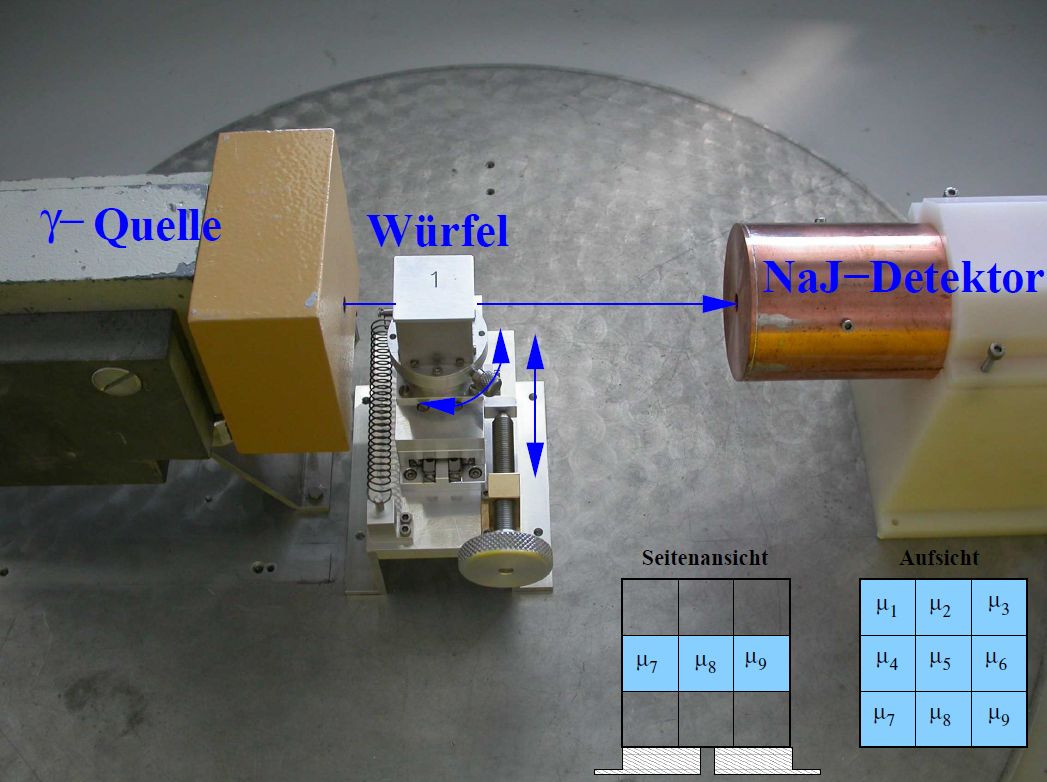
\includegraphics[height=7.0cm]{content/pictures/Aufbau.png}
  \caption{Darstellung des verwendeten Versuchsaufbaus.\cite{anleitung}}
  \label{fig:Aufbau}
\end{figure}
Zu Beginn des Versuchs wird der $\ce{^137Cs}$-Strahler durch den Assistenten, in den Versuchsaufbau aus Abbildung \ref{fig:Aufbau} eingebaut. 
Anschließend wird eine Nullmessung, dass bedeutet keine Probe im Strahlengang
aufgenummen. Dazu wird das Programm \textit{Maestro} verwendet, welches auf dem bereitgestellten Computer installiert ist. Dieses stellt die daten des 
Multichannel-Analyser graphisch da. Der Multichannel-Analyser ist an den Photo-Multiplier des Szintillationsdetektor angeschlossen, welcher die $\gamma$-Strahlung nachweist.
Anschließend wird nur ein Aluminiumgehäuse, welches die Würfel im Inneren zusammen hält vermessen. Dabei ist darauf zu achetn, dass für einen statistischen Fehler
von weniger als \SI{3}{\percent} eine Zählrate von \num{1112} erreicht werden muss, was sich nach der Poissonverteilung ergibt. Es werden insgasamt
zwölf Messungen mit einem Strahlenverlauf wie in Abbildung \ref{fig:wuerfel} dargestellt, durchgeführt.
Nun werden noch zwei Vollwürfel untersucht, welche ebenfalls durch ein Aluminumgehäuse geschützt sind. Dazu werden für beide nur vier Messungen benötigt,
da die jeweils anderen äquivalent sind.
Zuletzt wird noch ein Würfel, welcher aus \num{27} Einzelwürfeln besteht genauer untersucht. Der Aufbau lässt aber nur die Vermessung der mittleren Ebene zu, hier werden 
wieder alle zwölf Messungen durchgeführt.
\FloatBarrier
\newpage
\section{Auswertung}
\label{sec:Auswertung}
Die gesamte Auswertung wird mit Hilfe der Bibilotheken \cite{matplotlib}, \cite{numpy}, \cite{scipy} und
\cite{uncertainties} in \textit{python} durchgeführt. Bei den abgebildeten Spektren handelt es sich stets um 
Ausschnitte der gesamt Spektren, welche \num{8192} Kanäle besitzen. Es ist stets nur der markante Bereich
mit den relevanten Peaks dargestellt.


\subsection{Energiekalibration}
\label{sec:Energiekalibration}
Zu Beginn des Versuchs wird zunächst die Probe ${}^{152}$Eu untersucht. Die Messwerte
sind in Abbildung \ref{fig:Eu_log_Kanal} logarithmisch dargestellt.
Die für die Kalibrierung verwendeten Peaks sind mit roten Kreuzen makiert. Die Messwerte
werden mit den theoretischen Werten \cite{referenz1} verglichen, sodass mit Hilfe einer linearen Ausgleichsrechnung
eine Zuordnung von Kanalnummer $i$ und Energie $E$ möglich ist. Diese Daten sind
gemeinsam mit den Emissionswahrscheinlichkeit in Tabelle \ref{tab:zuordnung_eu}
gelistet, dabei werden Energien mit einer Emissionswahrscheinlichkeit $W$
kleiner als \SI{2}{\percent} vernachlässigt.
Da die Peaks einen Gauß-Glocken förmigen Verlauf haben, wird zunächst ein Gauß-Fit der Form
\begin{equation}
  N(i) = h \cdot \exp{\left(-\frac{\left(i - \mu\right)^2}{\sigma^2}\right)} + a
\end{equation}
über die identifizierten Peaks durchgeführt. Die Ergebnisse dieses Fits sind in Tabelle \ref{tab:gauss_parameter}
dargestellt, dabei bezeichnet $\mu$ den Mittelwert, $h$ die Höhe des Peaks, $\sigma$ die Standardabweichung und 
$a$ ein Parameter, welcher den Untergrund darstellt. Für den Fit wird der detektierte Kanal und die auf jeder Seite 
\num{40} nebenliegenden Kanäle verwendet. Anschließend wird mit der gefitteten Kanalnummer die Ausgleichsrechnung
durchgeführt. Für die Ausgleichsrechnung wird eine Gerade der Form
\begin{equation}
  E = m \cdot i + b
\end{equation}
verwendet, wobei $m$ die Steigung und $b$ der y-Achsenabschnitt ist. Dabei lassen sich die Parameter zu
\begin{gather*}
  m = \SI{0.40302(2)}{\kilo\electronvolt\per\kanal} \\
  b = \SI{-2.63(4)}{\kilo\electronvolt}
\end{gather*}
bestimmen.
In der Abbildung \ref{fig:kalibration} ist das Ergebnis der Ausgleichsrechnung graphisch
dargestellt, dabei befindet sich auf der x-Achse die Kanalnummer $i$ und auf der
y-Achse die errechnete Energie $E_\text{i}$.


\begin{figure}[htb]
 \centering
 \includegraphics[width=\textwidth]{Eu_log_Kanal.pdf}
 \caption{Die Zählrate $N$ in Abhängigkeit der Kanalnummer $i$ für ${}^{152}$Eu mit logarithmierter y-Skala.}
 \label{fig:Eu_log_Kanal}
\end{figure}

\begin{figure}[htb]
 \centering
 \includegraphics[width=\textwidth]{build/kalibration.pdf}
 \caption{Die ermittelte Energie anhand der Daten in Abhängigkeit der Kanalnummer zur Kalibartion des Ge-Detektors.}
 \label{fig:kalibration}
\end{figure}
\begin{table}
	\centering
	\caption{Gegebene Werte zur Kalibrierung des Germanium-Detektors \cite{referenz1}.}
	\label{tab:zuordnung_eu}
	\begin{tabular}{
		S[table-format=4.4] @{${}\pm{}$} S[table-format=1.4]
		S[table-format=2.3] @{${}\pm{}$} S[table-format=1.3]
		S[table-format=4.0]
		}
	\toprule
		\multicolumn{2}{c}{ $E_\text{i}$\;/\;\si{\kilo\electronvolt}} &
		\multicolumn{2}{c}{ $W_\text{i}$\;/\;\si{\percent}} &
		{$i$} \\
	\midrule
		 121.7817 &  0.0003 &  28.41 &  0.13 &  309 \\
		 244.6974 &  0.0008 &  7.55 &  0.04 &  614 \\
		 295.9387 &  0.0017 &  0.442 &  0.003 &  740 \\
		 344.2785 &  0.0012 &  26.59 &  0.12 &  861 \\
		 411.1165 &  0.0012 &  2.238 &  0.010 &  1027 \\
		 443.965 &  0.003 &  3.120 &  0.028 &  1108 \\
		 778.9045 &  0.0024 &  12.97 &  0.06 &  1939 \\
		 867.380 &  0.003 &  4.243 &  0.023 &  2159 \\
		 964.079 &  0.018 &  14.50 &  0.06 &  2399 \\
		 1085.837 &  0.010 &  10.13 &  0.06 &  2702 \\
		 1112.076 &  0.003 &  13.41 &  0.06 &  2765 \\
		 1408.013 &  0.003 &  20.85 &  0.08 &  3500 \\
	\bottomrule
	\end{tabular}
\end{table}
\begin{table}
	\centering
	\caption{Parameter des durchgeführten Gauss-Fits pro Kanal.}
	\label{tab:gauss_parameter}
	\begin{tabular}{
		S[table-format=4.0]
		S[table-format=4.3] @{${}\pm{}$} S[table-format=1.3]
		S[table-format=2.1] @{${}\pm{}$} S[table-format=1.1]
		S[table-format=4.0] @{${}\pm{}$} S[table-format=2.0]
		S[table-format=1.3] @{${}\pm{}$} S[table-format=1.3]
		}
	\toprule
		{$i$} &
		\multicolumn{2}{c}{$\mu_\text{i}$} &
		\multicolumn{2}{c}{$a_\text{i}$} &
		\multicolumn{2}{c}{$h_\text{i}$} &
		\multicolumn{2}{c}{$\sigma_\text{i}$} \\
	\midrule
		 309 &  308.773 &  0.005 &  98.8 &  2.6 &  5344 &  20 &  1.644 &  0.007 \\
		 614 &  613.758 &  0.015 &  44.6 &  1.1 &  757 &  7 &  1.941 &  0.022 \\
		 740 &  740.872 &  0.187 &  31.4 &  0.7 &   43 &  5 &  1.971 &  0.269 \\
		 861 &  860.839 &  0.007 &  24.8 &  1.0 &  1668 &  6 &  2.167 &  0.009 \\
		 1027 &  1026.680 &  0.054 &  20.1 &  0.6 &  118 &  3 &  2.283 &  0.079 \\
		 1108 &  1108.071 &  0.042 &  18.9 &  0.5 &  134 &  3 &  2.376 &  0.060 \\
		 1939 &  1939.059 &  0.046 &  15.2 &  0.7 &  202 &  3 &  3.351 &  0.067 \\
		 2159 &  2158.525 &  0.137 &  14.4 &  0.5 &   51 &  2 &  3.709 &  0.201 \\
		 2399 &  2398.434 &  0.046 &  8.1 &  0.5 &  160 &  2 &  4.206 &  0.068 \\
		 2702 &  2701.024 &  0.102 &  7.1 &  0.7 &  101 &  3 &  4.707 &  0.150 \\
		 2765 &  2765.719 &  0.080 &  6.2 &  0.6 &  115 &  2 &  4.825 &  0.118 \\
		 3500 &  3500.536 &  0.093 &  1.1 &  0.7 &  119 &  3 &  5.498 &  0.139 \\
	\bottomrule
	\end{tabular}
\end{table}
\FloatBarrier

\subsection{Vollenergienachweiseffizienz}
\label{sec:Vollenergienachweiseffizenz}
Die Aktivität der Probe am $15.04.2019$, dem Versuchstag lässt sich mit
\begin{equation}
  A = A_0 \cdot \exp{\left(-\lambda \cdot t\right)}
\end{equation}
berechnen, hierbei ist $A_0$ die Aktivität am Produktionstag,
$\lambda = \SI[per-mode = reciprocal-positive-first]{1.6244(19)e-9}{\per\second}$ \cite{referenz1} 
die Zerfallskonstante und $t$ die Zeit. Es ist aus \cite{V18} bekannt, dass die Probe am Produktionstag, dem
$01.10.2000$ eine Aktivität von $\SI{4130(60)}{\becquerel}$ besaß.
Die Aktivität am Versuchstag beläuft sich damit auf
\begin{equation*}
  \SI{1597(23)}{\becquerel}.
\end{equation*}
Des Weiteren lässt sich mit Hilfe der Formel \ref{eqn:raum} der Raumwinkel errechnen.
Dabei beträgt $a~=~\SI{8.8(1)}{\centi\meter}$, was sich aus dem Abstand der Probe zum
Aluminiumgehäuse (\SI{7.3(1)}{\centi\meter}) und dem Abstand des Gehäuses zum Detektor 
(\SI{1.5}{\centi\meter}) ergibt. Der Radius $r$ des Detektors betrug \SI{2.25}{\centi\meter}, was sich
aus der Abbildung \ref{fig:Detektor} ablesen lässt. Damit lässt sich der Raumwinkel zu
\begin{equation*}
  \frac{\Omega}{4\pi} = \num{0.0156(3)}
\end{equation*}
bestimmen.
Unter Zuhilfenahme von
\begin{equation}
  Z_\text{i} = \sqrt{2\pi} h_\text{i} \sigma_{i}
\end{equation}
lässt sich der Peakinhalt $Z_\text{i}$ bestimmen. Nun lässt sich mit Formel \ref{eqn:eff}
die Nachweiswahrscheinlichkeit des Detektors errechnen. Dabei ist die Messzeit von $t_\text{mess} = \SI{4676}{\second}$
zu berücksichtigen. Die sich ergeben Werte sind in Tabelle \ref{tab:det_eff} gelistet.
Anhand der Werte aus Tabelle \ref{tab:det_eff} lässt sich ein Fit der Form
\begin{equation}
  \label{eqn:Potenz}
  Q(E) = a \cdot \left(\frac{E-b}{\SI{1}{\kilo\electronvolt}}\right)^c + d
\end{equation}
durchführen. Dabei werden nur Peaks der Energie $E_\text{i} > \SI{150}{\kilo\electronvolt}$ berücksichtigt,
da nur hier gegebenen ist, dass sie die Aluminiumhaube und die äußere Schicht des Detektors nahezu
ungehindert durchdringen. Die Parameter ergeben sich dabei zu
\begin{align*}
  a &= \num{-0.01(11)} \\
  b &= \SI{121.81(5)}{\kilo\electronvolt} \\
  c &= \num{0.4(8)} \\
  d &= \num{0.4(5)}.
\end{align*}
Eine graphische Darstellung dieser Ausgleichsrechnung ist in Abbildung \ref{fig:effizenz} zu finden.

\begin{figure}[htb]
 \centering
 \includegraphics[width=\textwidth]{build/efficiency.pdf}
 \caption{Die Vollenergienachweiseffizienz des Detektors gegen die Energie aufgetragen.}
 \label{fig:effizenz}
\end{figure}
\begin{table}
	\centering
	\caption{Peakinhalt, Energie und Detektoreffizenz als Ergebnis des Gaußfits.}
	\label{tab:det_eff}
	\begin{tabular}{
		S[table-format=4.2] @{${}\pm{}$} S[table-format=1.2]
		S[table-format=2.3] @{${}\pm{}$} S[table-format=1.3]
		S[table-format=5.0] @{${}\pm{}$} S[table-format=3.0]
		S[table-format=1.3] @{${}\pm{}$} S[table-format=1.3]
		}
	\toprule
		\multicolumn{2}{c}{$E_\text{i}$\;/\;\si{\kilo\electronvolt}} &
		\multicolumn{2}{c}{$W_\text{i}$\;/\;\si{\percent}} &
		\multicolumn{2}{c}{$Z_\text{i}$\;/\;\si{\kilo\electronvolt}} &
		\multicolumn{2}{c}{$Q_\text{i}$\;/\;\si{\becquerel }} \\
	\midrule
		 121.81 &  0.04 &  28.41 &  0.13 &  22027 &  124 &  0.666 &  0.018 \\
		 244.73 &  0.05 &  7.55 &  0.04 &  3685 &  55 &  0.419 &  0.013 \\
		 295.96 &  0.09 &  0.442 &  0.003 &   211 &  38 &  0.41 &  0.08 \\
		 344.30 &  0.05 &  26.59 &  0.12 &  9061 &  52 &  0.293 &  0.008 \\
		 411.14 &  0.05 &  2.238 &  0.010 &   674 &  31 &  0.259 &  0.014 \\
		 443.94 &  0.05 &  3.12 &  0.03 &   798 &  26 &  0.220 &  0.009 \\
		 778.84 &  0.06 &  12.97 &  0.06 &  1699 &  45 &  0.113 &  0.004 \\
		 867.29 &  0.08 &  4.24 &  0.02 &   477 &  34 &  0.097 &  0.007 \\
		 963.98 &  0.07 &  14.50 &  0.06 &  1686 &  36 &  0.100 &  0.003 \\
		 1085.93 &  0.08 &  10.13 &  0.06 &  1193 &  50 &  0.101 &  0.005 \\
		 1112.00 &  0.08 &  13.41 &  0.06 &  1387 &  44 &  0.089 &  0.004 \\
		 1408.14 &  0.10 &  20.85 &  0.08 &  1640 &  54 &  0.068 &  0.003 \\
	\bottomrule
	\end{tabular}
\end{table}
\FloatBarrier


\subsection{Detektoreigenschaften}
\label{sec:Detektoreigenschaften}
Um die Detektoreigenschaften genauer zu untersuchen wird das Spektrum von ${}^{137}$Cs über eine Zeit
von $t_\text{mess} = \SI{3365}{\second}$ aufgenommen. Wie in Abbildung \ref{fig:Cs_log} zu erkennen, besitzt Cäsium
ein monochromatisches Spektrum. Im Folgendem wird dieser und die beiden anderen Charakteristika, der Rückstreupeak
sowie die Comptonkante näher untersucht. Die detektierten Peaks sind in Tabelle \ref{tab:zuordnung_Cs} zugeordnet. 
Die theoretischen Emissionsenergie des Cäsium liegt bei \SI{661.657(3)}{\kilo\electronvolt} \cite{referenz1}. Mit Hilfe
ihrer, kann nach Formel \ref{eqn:Com_Kante} der theoretische Wert der Comptonkante auf $\SI{477.27}{\kilo\electronvolt}$
bestimmt werden. Des Weiteren lässt sich nach Formel \ref{eqn:rueck} auch der theoretische Wert für den Rückstreupeak
auf \SI{184.32}{\kilo\electronvolt} ermitteln. Der Wert von $m_\text{e} c^2 = \SI{510.9989461(31)}{\kilo\electronvolt}$ wird 
der Referenz \cite{codata} entnommen. 
\begin{figure}[htb]
 \centering
 \includegraphics[width=\textwidth]{build/Cs_log.pdf}
 \caption{Das aufgenommene Spektrum des ${}^{137}$Cs-Strahlers in Abhängigkeit der Energie mit logarithmierter y-Achse.}
 \label{fig:Cs_log}
\end{figure}
\begin{table}
	\centering
	\caption{Zuordnung der detektierten Peaks von Cäsium.}
	\label{tab:zuordnung_Cs}
	\begin{tabular}{
		c
		S[table-format=4.0]
		S[table-format=3.2] @{${}\pm{}$} S[table-format=1.3]
		}
	\toprule
		{} &
		{Index $i$} &
		\multicolumn{2}{c}{$E_\text{i, ist}$\;/\;\si{\kilo\electronvolt}} \\
	\midrule
		 Rückstreupeak &  471	&	187.20 & 1.4	\\
		 Comptonkante &  1166	&	467.29 &	1.4	\\
		 Vollenergiepeak &  1649	&	661.562	& 0.007\\
	\bottomrule
	\end{tabular}
\end{table}
Dabei wird die Energie der Comptonkante aus der Abbildung \ref{fig:Cs_log} abgelesen, ebenso wie für den 
Rückstreupeak. Für das Ablesen wir eine Genauigkeit von \num{3} Kanälen angenommen.
Für den Vollenergiepeak wir erneut wie in Abschnitt \ref{sec:Energiekalibration} ein Gauß-Fit durchgeführt.
Die Parameter ergeben sich zu
\begin{align*}
  \mu &= \SI{661.562(7)}{\kilo\electronvolt} \\
  \sigma &= \SI{1.259(10)}{\kilo\electronvolt} \\
  h &= \num{2167(15)} \\
  a &= \num{4(3)}.
\end{align*}

Eine weiter wichtige Größe des Detektors ist Halbwertsbreite $E_{\sfrac{1}{2}}$, welche ein Maß für das Auflösungsvermögen ist
und den Ge-Detektor auszeichnet. Diese, sowie die Zehntelbreite $E_{\sfrac{1}{10}}$ lassen sich aus Abbildung \ref{fig:Halb} ablesen, 
dabei ergibt sich 
\begin{gather*}
  E_{\sfrac{1}{2}} = \SI{2.20(10)}{\kilo\electronvolt} \\
  E_{\sfrac{1}{10}} = \SI{3.90(10)}{\kilo\electronvolt}.
\end{gather*}
Bei den angegebenen Fehlern handelt es sich um Ablesefehler aus der Abbildung \ref{fig:Halb}.
Der Quotient dieser beiden Größen ist ein Maß für das Energieauflösungsvermögen des Detektors. Der hier ermittelte 
Quotient der gemessenen Größen beläuft sich auf
\begin{equation*}
  \frac{E_{\sfrac{1}{10}}}{E_{\sfrac{1}{2}}} = \SI{1.77(9)}{\kilo\electronvolt}.
\end{equation*}

Die theoretischen Werte ergeben sich aus der Standardabweichung $\sigma$ des Fits. Da aber nur der Quotient interessiert, 
kürzt sich diese und es ergibt sich
\begin{equation}
  \frac{E_{\sfrac{1}{10}}}{E_{\sfrac{1}{2}}} = \frac{\sqrt{8 \cdot \log{(10)}} \cdot \sigma_\text{fit}}{\sqrt{8 \cdot \log{(2)}} \cdot \sigma_\text{fit}} = \sqrt{\frac{\log{(10)}}{\log{(2)}}} = \num{1.823}
\end{equation}
als theoretischer Wert.
\begin{figure}[htb]
 \centering
 \includegraphics[width=\textwidth]{build/vollpeak.pdf}
 \caption{Der Vollenergiepeak des Cäsium zur Bestimmung der Halbwerts-/Zehntelsbreite.}
 \label{fig:Halb}
\end{figure}

Der Vollenergiepeak kann maßgeblich durch den Photo- und Comptoneffekt entstehen. Mit Hilfe der Formel \ref{eq:Absorbtion} und 
der Extinktionskoeffizienten, welche aus Abbildung \ref{fig:Germanium} abgelesen werden, lassen sich die Absorptionswahrscheinlichkeiten
zu
\begin{align*}
  p_\text{Ph} = \SI{2.7(11)}{\percent} \\
  p_\text{Com} = \SI{75(7)}{\percent}
\end{align*}
bestimmen.
Die Extinktionskoeffizienten lassen sich auf 
\begin{gather*}
  \mu_\text{Ph} = \SI{0.007(3)}{\per\centi\meter} \\
  \mu_\text{Com} = \SI{0.37(7)}{\per\centi\meter}
\end{gather*}
bestimmen, die Länge des Detektors wurde aus Abbildung \ref{fig:Detektor} entnommen und beträgt \SI{3.9}{\centi\meter}.
Das Verhältnis der Absorptionwahrscheinlichkeiten beträgt $\num{28(12)}$.
Der Inhalt des Vollenergiepeaks lässt sich bestimmen, in dem analog zu Abschnitt \ref{sec:Vollenergienachweiseffizenz} 
vorgegangen wird. Dabei werden die auf beiden Seiten nächstliegenden \num{50} Kanäle verwendet.
Für das Comptonkontiuums wird die numerischen Integration im Bereich von
\SIrange{18.70}{467.27}{\kilo\electronvolt} verwendet. Der Inhalt beträgt für den
Vollenergiepeak \SI{3.89(7)e4}{\kilo\electronvolt} und für das Comptonkontiuum \SI{1.75(14)e5}{\kilo\electronvolt}. 
Berechnung des Verhältnis der Inhalte ergibt einen Wert von $\num{106(8)}$.
\FloatBarrier

\subsection{Aktivitätsbestimmung}
\label{sec:Aktiv}
In der Abbildung \ref{fig:mystery1} ist das Spektrum eines Strahlers dargestellt. Es soll herausgefunden werden,
ob es sich um ${}^{133}$Ba oder ${}^{125}$Sb handelt, dafür wird die Aktivität der Peaks bestimmt. Dazu werden
die Peaks dem passendem Spektrum mit ihrer Emissionswahrscheinlichkeit zugeordnet, was in Tabelle \ref{tab:zuordnung_Ba}
dargestellt ist. Der Vergleich mit der Literatur \cite{referenz1} zeigt, dass es sich um Barium handelt. 
Die Emissionswahrscheinlichkeiten werden der Referenz \cite{referenz1} entnommen um damit die Aktivität zu bestimmen. 
Des Weiteren wird der Inhalt der Peaks bestimmt und mit Hilfe der Formel 
\ref{eqn:eff} die Aktivität errechnet. Mit der Messzeit von \SI{3205}{\second} ergeben sich die Werte in Tabelle 
\ref{tab:aktivitaet_ba}. Die verwendeten Parameter des durchgeführten Gauß-Fits ergeben sich zu den in Tabelle \ref{tab:Ba} 
gegebenen Werten. Die gemittelte Aktivität ergibt sich zu
\begin{equation*}
  A = \SI{1.32(17)e3}{\becquerel}.
\end{equation*}
\begin{table}
	\centering
	\caption{Die Zuordnung zum Spektrum des ${}^{133}$Ba \cite{referenz1}.}
	\label{tab:zuordnung_Ba}
	\begin{tabular}{
		S[table-format=3.4] @{${}\pm{}$} S[table-format=1.4]
		S[table-format=2.3] @{${}\pm{}$} S[table-format=1.3]
		S[table-format=3.0]
		S[table-format=3.2] @{${}\pm{}$} S[table-format=1.2]
		}
	\toprule
		\multicolumn{2}{c}{$E_\text{theo}$\;/\;\si{\kilo\electronvolt}} &
		\multicolumn{2}{c}{$W_\text{i}$\;/\;\si{\%}} &
		{$i$} &
		\multicolumn{2}{c}{$E_\text{fit}$\;/\;\si{\kilo\electronvolt}} \\
	\midrule
		 53.1622 &  0.0018 &  2.14 &  0.06 &  138 &  52.99 &  0.04 \\
		 79.6142 &  0.0019 &  2.63 &  0.19 &  194 &  75.56 &  0.04 \\
		 80.9979 &  0.0011 &  33.31 &  0.30 &  208 &  81.20 &  0.04 \\
		 160.6121 &  0.0016 &  0.638 &  0.006 &  405 &  160.59 &  0.04 \\
		 223.2368 &  0.0013 &  0.450 &  0.005 &  560 &  223.06 &  0.04 \\
		 302.8508 &  0.0005 &  18.31 &  0.11 &  758 &  302.86 &  0.05 \\
		 356.0129 &  0.0007 &  62.05 &  0.19 &  890 &  356.06 &  0.05 \\
		 383.8485 &  0.0012 &  8.94 &  0.06 &  959 &  383.86 &  0.05 \\
	\bottomrule
	\end{tabular}
\end{table} 
\begin{table}
	\centering
	\caption{Berechnete Aktivität der betrachteten Emissionslinien mit dazu korrespondierenden Detektor-Effizienzen.}
	\label{tab:aktivitaet_ba}
	\begin{tabular}{
		S[table-format=3.2] @{${}\pm{}$} S[table-format=1.2]
		S[table-format=2.3] @{${}\pm{}$} S[table-format=1.3]
		S[table-format=1.4] @{${}\pm{}$} S[table-format=1.4]
		S[table-format=5.0] @{${}\pm{}$} S[table-format=2.0]
		S[table-format=4.0] @{${}\pm{}$} S[table-format=3.0]
		}
	\toprule
		\multicolumn{2}{c}{$E_\text{i}$\;/\;\si{\kilo\electronvolt}} &
		\multicolumn{2}{c}{$W_\text{i}$\;/\;\si{\percent}} &
				\multicolumn{2}{c}{$Q_\text{i}$} &
		\multicolumn{2}{c}{$Z_\text{i}$\;/\;\si{\kilo\electronvolt}} &
		\multicolumn{2}{c}{$A_\text{i}$\;/\;\si{\becquerel}} \\
	\midrule
		 223.27 &  0.20 &  0.450 &  0.005 & 1.7 &  0.7 &   109 &  48 &  1810 &  793 \\
		 302.93 &  0.05 & 18.31 &  0.11 &  0.0511 &  0.0018 &  3733 &  33 &  1708 &  41 \\
		 356.06 &  0.05 & 62.05 &  0.19 &  0.0358 &  0.0010 &  10592 &  59 &  1533 &  35 \\
		 383.91 &  0.05 &  8.94 &  0.06 & 0.072 &  0.005 &  1426 &  14 &  1482 &  37 \\
	\bottomrule
	\end{tabular}
\end{table}
\begin{table}
	\centering
	\caption{Parameter des Gauß-Fits für das gegeben Spektrum}
	\label{tab:Ba}
	\begin{tabular}{
		S[table-format=3.2] @{${}\pm{}$} S[table-format=1.2]
		S[table-format=4.1e1] @{${}\pm{}$} S[table-format=2.1e1]
		S[table-format=2.3e1] @{${}\pm{}$} S[table-format=1.3e1]
		}
	\toprule
		\multicolumn{2}{c}{$\mu_\text{i}$\;/\;\si{\kilo\electronvolt}} &
		\multicolumn{2}{c}{$h_\text{i}$} &
		\multicolumn{2}{c}{$\sigma_\text{i}$\;/\;\si{\kilo\electronvolt}} \\
	\midrule
		 52.72 &  3.10 &  61 &  3 &  5e1 &  3e1 \\
		 80.93 &  0.10 &  276e1 &  8e1 &  1.14 &  0.04 \\
		 155.0 &  2.4 &  92 &  4 &  29 &  7 \\
		 222.2 &  1.0 &  31.1 &  1.7 &  25 &  5 \\
		 276.41 &  0.11 &  330 &  10 &  1.48 &  0.05 \\
		 302.87 &  0.11 &  743 &  9 &  1.462 &  0.020 \\
		 356.00 &  0.11 &  1972 &  11 &  1.525 &  0.009 \\
		 383.85 &  0.11 &  253.8 &  2.7 &  1.619 &  0.020 \\
	\bottomrule
	\end{tabular}
\end{table}
\begin{figure}[htb]
 \centering
 \includegraphics[width=\textwidth]{build/mystery1_log.pdf}
 \caption{Das Spektrum des zu bestimmenden Strahlers(${}^{133}$Ba oder ${}^{125}$Sb).}
 \label{fig:mystery1}
\end{figure}
\FloatBarrier


\subsection{Unbekanntes Salz}
\label{sec:Salz}
Es soll nun das Spektrum eines unbekannten Strahlers untersucht werden. Hierzu wird das in Abbildung \ref{fig:Salz}
dargestellte Spektrum, welches über eine Zeit von \SI{4510}{\second} gemessen wurde näher untersucht.
Als erstes werden die auftretenden Peaks identifiziert, diese sind in Tabelle \ref{tab:Salz} dargestellt.
Mit Hilfe von \cite{referenz1} werden diese identifiziert und ihrem Emissionselement zugeordnet. Die Zuordnung ist
ebenfalls in der Tabelle \ref{tab:Salz} zu erkennen.
In Tabelle \ref{tab:aktivitaet_e} lassen sich die ermittelten Werte zur Bestimmung der Aktivität einsehen.
Die mittleren Aktivitäten der Nuklide lassen sich auf
\begin{align*}
  A_\text{Ra} & = \SI{6.3(2)e3}{\becquerel} \\
  A_\text{Pd} & = \SI{5.6(10)e3}{\becquerel} \\
  A_\text{Bi} & = \SI{3.74(17)e3}{\becquerel}
\end{align*}
bestimmen. Dabei werden nur die Werte im Bereich der \SIrange{150}{1700}{\kilo\electronvolt} verwendet, 
da nur in diesem Bereich die Effizienz nach Abschnitt \ref{sec:Vollenergienachweiseffizenz} ihre Gültigkeit besitzt.
Auf Grund der auftretenden Elemente lässt sich auf die Zerfallsreihe
von ${}^{238}$Ur schließen, was mit \cite{referenz1} bestätigt wird.
\begin{table}
	\centering
	\caption{Die ermittelten Peaks zur Nuklid Bestimmung.}
	\label{tab:Salz}
	\begin{tabular}{
		S[table-format=4.3] @{${}\pm{}$} S[table-format=1.3]
		S[table-format=2.3] @{${}\pm{}$} S[table-format=1.3]
		S[table-format=4.0]
		S[table-format=4.2] @{${}\pm{}$} S[table-format=1.2]
		}
	\toprule
		\multicolumn{2}{c}{$E_\text{i}$\;/\;\si{\kilo\electronvolt}} &
		\multicolumn{2}{c}{$W_\text{i}$\;/\;\si{\percent}} &
		{$i$} &
		\multicolumn{2}{c}{$E_\text{i,fit}$\;/\;\si{\kilo\electronvolt}} \\
	\midrule
		 \multicolumn{7}{c}{\textbf{${}^{234}$Th}} \\
		 63.30 &  0.02 &  3.75 &  0.08 &  164 &  63.47 &  0.04 \\
		 92.38 &  0.01 &  2.18 &  0.19 &  236 &  92.48 &  0.04 \\
		 \multicolumn{7}{c}{\textbf{${}^{226}$Ra} }\\
		 186.211 &  0.013 &  3.555 &  0.019 &  468 &  185.98 &  0.04 \\
		 665.453 &  0.022 &  1.530 &  0.007 &  1657 &  665.17 &  0.06 \\
		 1847.420 &  0.025 &  2.025 &  0.012 &  4594 &  1848.83 &  0.11 \\
		 2118.55 &  0.03 &  1.158 &  0.005 &  5266 &  2119.65 &  0.12 \\
		 \multicolumn{7}{c}{\textbf{${}^{214}$Pb}} \\
		 \multicolumn{2}{c}{\num{77.1088}} &  10.47 &  0.20 &  198 &  77.17 &  0.04 \\
		 \multicolumn{2}{c}{\num{87.347}}  &  3.59 &  0.09 &  223 &  87.25 &  0.04 \\
		 241.997 &  0.003 &  7.268 &  0.022 &  607 &  242.00 &  0.04 \\
		 295.224 &  0.002 &  18.414 &  0.036 &  739 &  295.20 &  0.05 \\
		 351.932 &  0.002 &  35.60 &  0.07 &  880 &  352.03 &  0.05 \\
		 785.96 &  0.09 &  1.064 &  0.013 &  1956 &  785.67 &  0.06 \\
		 1155.19 &  0.02 &  1.635 &  0.007 &  2874 &  1155.64 &  0.08 \\
		 1238.111 &  0.012 &  5.831 &  0.014 &  3078 &  1237.85 &  0.08 \\
		 1280.96 &  0.02 &  1.435 &  0.006 &  3184 &  1280.57 &  0.08 \\
		 1407.98 &  0.04 &  2.389 &  0.008 &  3499 &  1407.52 &  0.09 \\
		 1509.228 &  0.015 &  2.128 &  0.010 &  3752 &  1509.49 &  0.09 \\
		 1661.28 &  0.06 &  1.048 &  0.009 &  4130 &  1661.83 &  0.10 \\
		 1729.595 &  0.015 &  2.844 &  0.010 &  4300 &  1730.34 &  0.10 \\
		 2204.21 &  0.04 &  4.913 &  0.023 &  5475 &  2203.88 &  0.13 \\
		 \multicolumn{7}{c}{\textbf{${}^{214}$Bi}} \\
		 609.312 &  0.007 &  45.49 &  0.19 &  1518 &  609.15 &  0.05 \\
		 665.453 &  0.022 &  1.530 &  0.007 &  1657 &  665.17 &  0.06 \\
		 768.356 &  0.010 &  4.892 &  0.016 &  1912 &  767.94 &  0.06 \\
		 934.061 &  0.012 &  3.10 &  0.01 &  2324 &  933.98 &  0.07 \\
		 1120.287 &  0.010 &  14.91 &  0.03 &  2788 &  1120.98 &  0.07 \\
		 1377.669 &  0.012 &  3.968 &  0.011 &  3424 &  1377.30 &  0.09 \\
		 1764.494 &  0.014 &  15.31 &  0.05 &  4386 &  1765.00 &  0.11 \\
	\bottomrule
	\end{tabular}
\end{table}
\begin{table}
	\centering
	\caption{Berechnete Aktivität der betrachteten Emissionslinien mit dazu korrespondierenden Detektor-Effizienzen.}
	\label{tab:aktivitaet_e}
	\begin{tabular}{
		S[table-format=4.3] @{${}\pm{}$} S[table-format=1.3]
		S[table-format=2.3] @{${}\pm{}$} S[table-format=1.3]
		S[table-format=5.0] @{${}\pm{}$} S[table-format=3.0]
		S[table-format=1.3]
		S[table-format=5.0] @{${}\pm{}$} S[table-format=4.0]
		}
	\toprule
		\multicolumn{2}{c}{$E_\text{i}$\;/\;\si{\kilo\electronvolt}} &
		\multicolumn{2}{c}{$W_\text{i}$\;/\;\si{\percent}} &
		\multicolumn{2}{c}{$Z_\text{i}$\;/\;\si{\kilo\electronvolt}} &
		{$Q_\text{i}$} &
		\multicolumn{2}{c}{$A_\text{i}$\;/\;\si{\becquerel}} \\
	\midrule
		 186.211 &  0.013 &  3.555 &  0.019 &  6835 &  178 &  0.288 &  9496 &  326 \\
		 665.453 &  0.022 &  1.530 &  0.007 &   507 &  49 &  0.157 &  3011 &  300 \\
		 241.997 &  0.003 &  7.268 &  0.022 &  6958 &  165 &  0.261 &  5219 &  168 \\
		 295.224 &  0.002 &  18.414 &  0.036 &  14796 &  139 &  0.241 &  4735 &  112 \\
		 351.932 &  0.002 &  35.60 &  0.07 &  24499 &  294 &  0.224 &  4369 &  109 \\
		 785.96 &  0.09 &  1.064 &  0.013 &   397 &  70 &  0.137 &  3871 &  685 \\
		 1155.19 &  0.020 &  1.635 &  0.007 &   259 &  60 &  0.087 &  2585 &  597 \\
		 1238.111 &  0.012 &  5.831 &  0.014 &  1261 &  139 &  0.078 &  3966 &  445 \\
		 1280.96 &  0.02 &  1.435 &  0.006 &   232 &  63 &  0.073 &  3164 &  868 \\
		 1407.98 &  0.04 &  2.389 &  0.008 &   364 &  74 &  0.059 &  3679 &  754 \\
		 1509.228 &  0.015 &  2.128 &  0.010 &   645 &  225 &  0.049 &  8881 &  3109 \\
		 1661.28 &  0.06 &  1.048 &  0.009 &   374 &  207 &  0.034 &  15070 &  8357 \\
		 609.312 &  0.007 &  45.49 &  0.19 &  18042 &  321 &  0.167 &  3387 &   95 \\
		 665.453 &  0.022 &  1.530 &  0.007 &   507 &  49 &  0.157 &  3011 &  300 \\
		 768.356 &  0.010 &  4.892 &  0.016 &  1597 &  123 &  0.140 &  3324 &  266 \\
		 934.061 &  0.012 &  3.100 &  0.010 &   766 &  58 &  0.116 &  3044 &  241 \\
		 1120.287 &  0.010 &  14.91 &  0.03 &  3821 &  251 &  0.091 &  3986 &  276 \\
		 1377.669 &  0.012 &  3.968 &  0.011 &   987 &  130 &  0.062 &  5692 &  762 \\
	\bottomrule
	\end{tabular}
\end{table}
\begin{figure}[htb]
 \centering
 \includegraphics[width=\textwidth]{build/Uran.pdf}
 \caption{Das Spektrum eines unbekannten Nuklids.}
 \label{fig:Salz}
\end{figure}

% \subsection{Unterkapiel}
% \label{sec:Unterkapitel}

% \begin{figure}
%   \centering
%   \includegraphics[width=\textwidth]{Plot.pdf}
%   \caption{Bildunterschrift}
%   \label{fig:Plot1}
% \end{figure}

\section{Diskussion}
\label{sec:Diskussion}
Nach dem Abzug des ermittelten Untergrunds werden einige Werte kleiner als Null, sodass in den \eqref{eqn:int} und \eqref{eqn:lin2} Beträge
verwendet wurden. Ebenso wurde erst nach Abzug der verwendete Bereich und das Maximum festgelegt.

Für die ermittelten Aktivierungsenergien im Abschnitt \ref{sec:klT} ergibt sich für die Heizrate von etwa \SI{1}{\per\kelvin} eine 
Abweichung von \SI{7}{\percent} zum Literaturwert $W=\SI{0.66(1)}{\electronvolt} = \SI{1.06(2)e-19}{\joule}$ \cite{quelle}.
Für die Heizrate von  etwa \SI{2}{\per\kelvin} eine Abweichung von \SI{45}{\percent}. 
Die Abweichungen für die Aktivierungsenergien, welche in Abschnitt \ref{sec:grT} über den Polarisationsansatz ermittelt werden sind mit
\SI{29}{\percent} für die Heizrate von etwa \SI{1}{\per\kelvin} und \SI{46}{\percent} für die andere, größer. Dies 
widerspricht den Erwartungen, hier eine genauere Messung zu erhalten. Ein Grund für die großen Abweichungen
bei der Intgralmethode hat ihren Ursprung wohl in der nummerischen Berechnung der Werte.

Da die Abweichung der Relaxationszeit $\tau_0$ vom Literaturwert $\tau_0 = \SI{4(2)e-14}{\second}$ um mehrere Größenordnungen
abweicht, wird eine Errechnung der Abweichung als nicht sinnvoll betrachtet.
Diese Abweichungen können zum teil damit begründet werden, dass die Probe hydroskopisch ist 
und somit Wasser aufnimmt. Dies führt nicht nur zu einer Veränderung der Struktur als solches, sondern da Wasser selbst ein 
Dipol ist zu einer deutlichen Verfäschung der Messergebnisse. Die Ursache darin liegt, dass die Probe sich in keinem 
Ultrahochvakuum befand, sondern nur in einem Vorvakuum von etwa \SI{19}{\milli\bar}. 
Weitere Gründe sind die geringen fließenden Ströme, welche stark auf elektrische und magnetische Feldänderungen reagieren, sowie
die nicht konstante Heizrate, welche besonders für die Soll-Heizrate von \SI{2}{\kelvin\per\minute} starke Abweichungen zeigte, dies 
spiegelt sich auch in den Fehlern wieder, da hier die Abweichungen größer als für die kleinere Heizrate sind.


Das höhere erste Maximum in Abbildung \ref{fig:Messdaten2} im Bezug zum ersten Maximum in Abbildung \ref{fig:Messdaten1}, lässt
sich dadurch erklären, dass für einen schnelleren Temeperaturanstieg mehr Dipole gleichzeitig relaxaxieren. Denn die Relaxationszeit
ist nach Formel \eqref{ref:Relaxzeit} bekanntlich exponentiell von der reziproken Temperatur abhängig.
Die Position des Maximums verschiebt sich des Weiteren für höhere Heizraten zu höheren Temperaturen, da der Temeperaturanstieg
schneller abläuft, als dass die Dipole direkt folgen könnten und sich wieder statistisch verteilen.



\nocite{*}
\printbibliography

\section{Anhang}
\label{sec:Anhang}
\begin{figure}[htb]
  \centering
  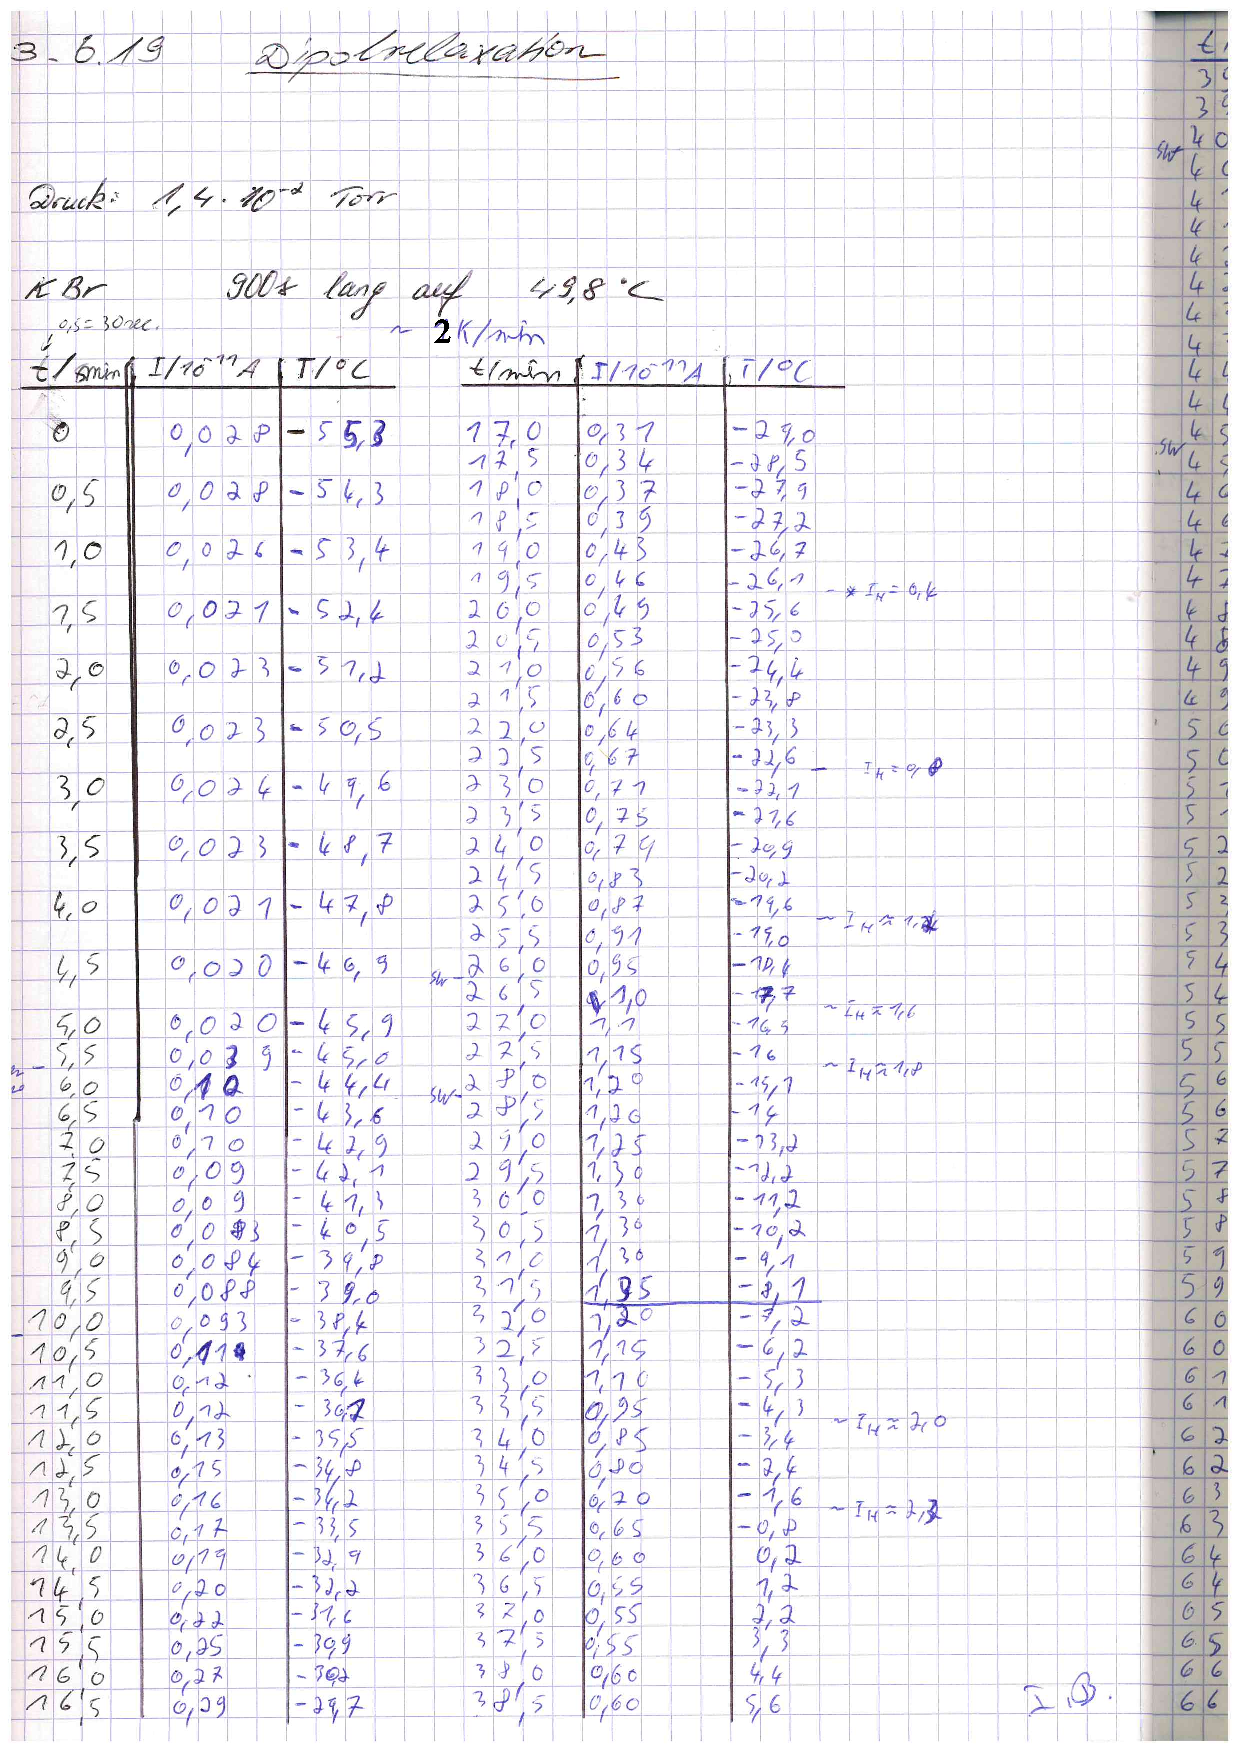
\includegraphics[height=\textheight]{data/Messdaten1.pdf}
\end{figure}
\begin{figure}[htb]
  \centering
  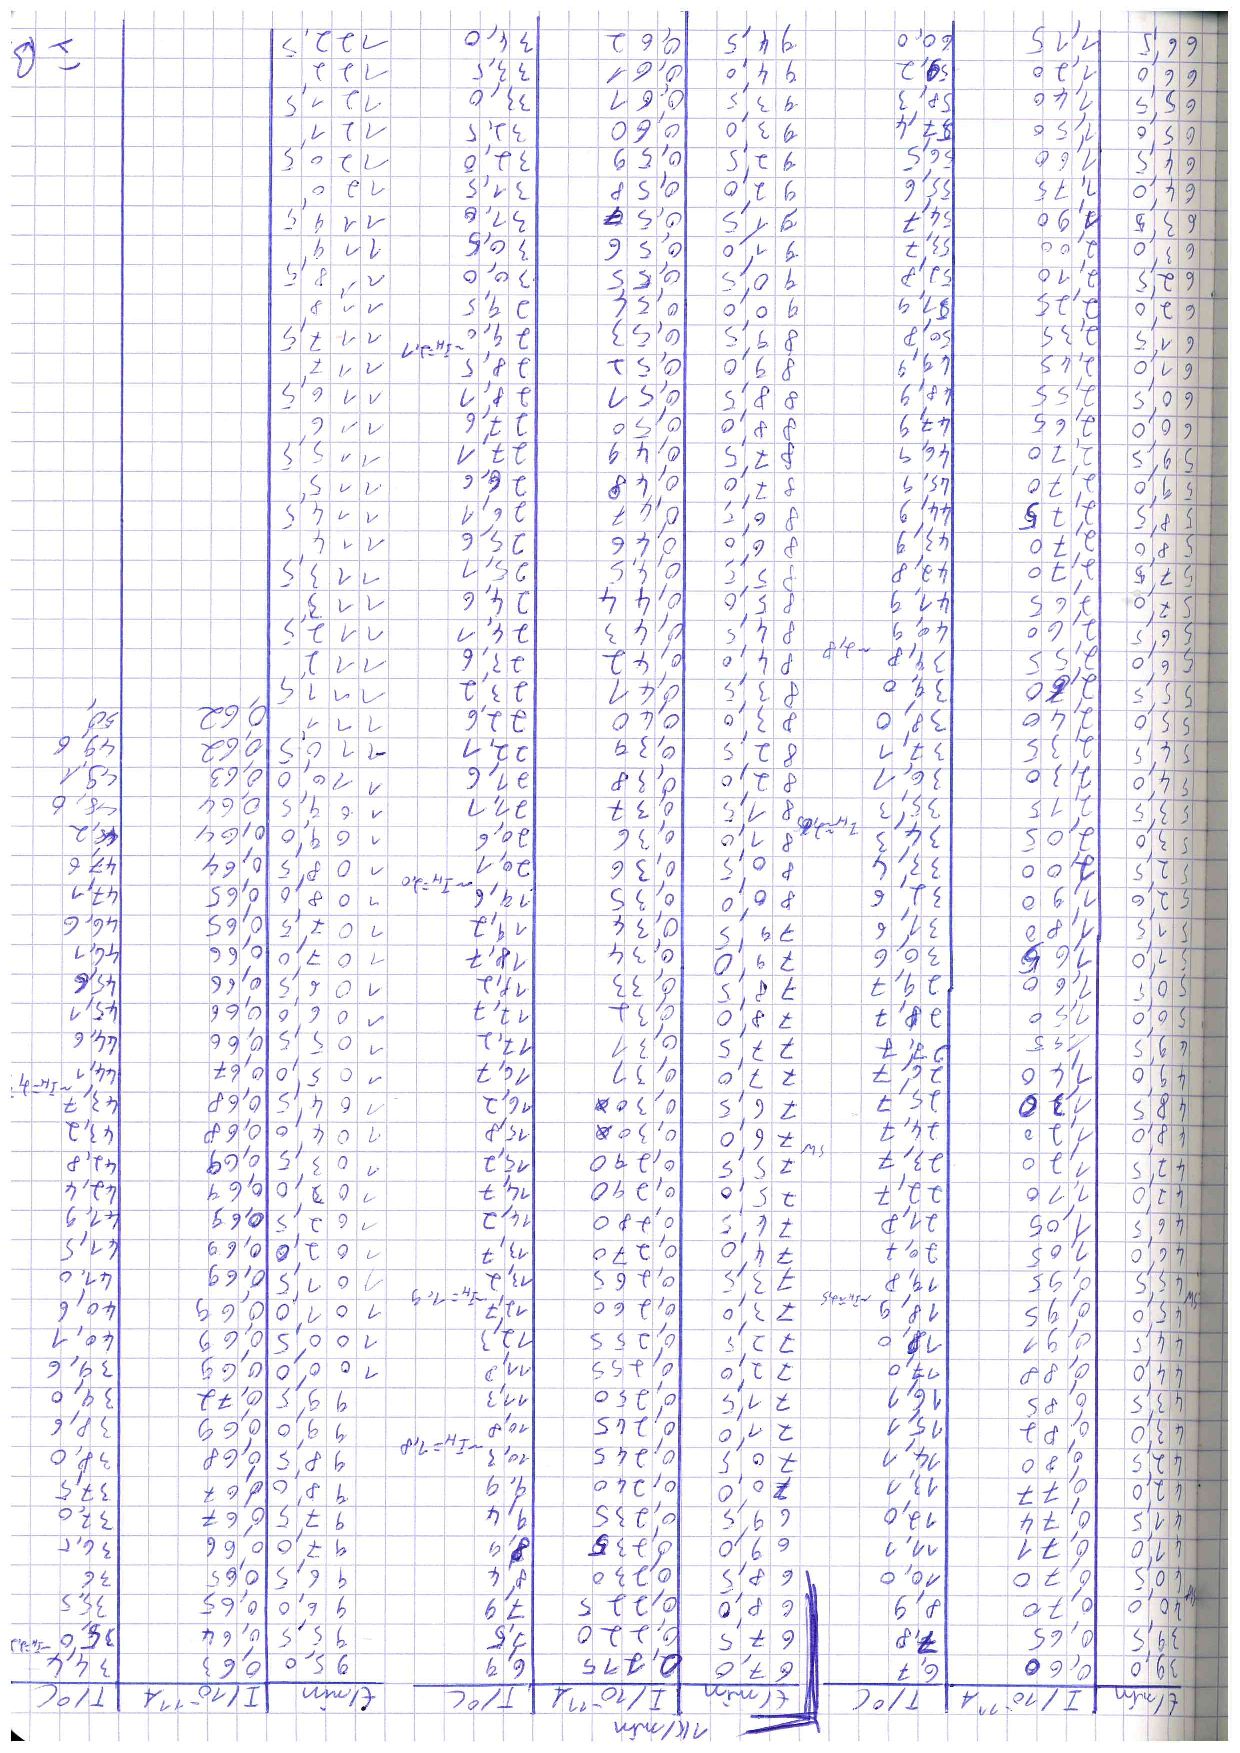
\includegraphics[height=\textheight, angle=180]{data/Messdaten2.pdf}
\end{figure}
\begin{figure}[htb]
  \centering
  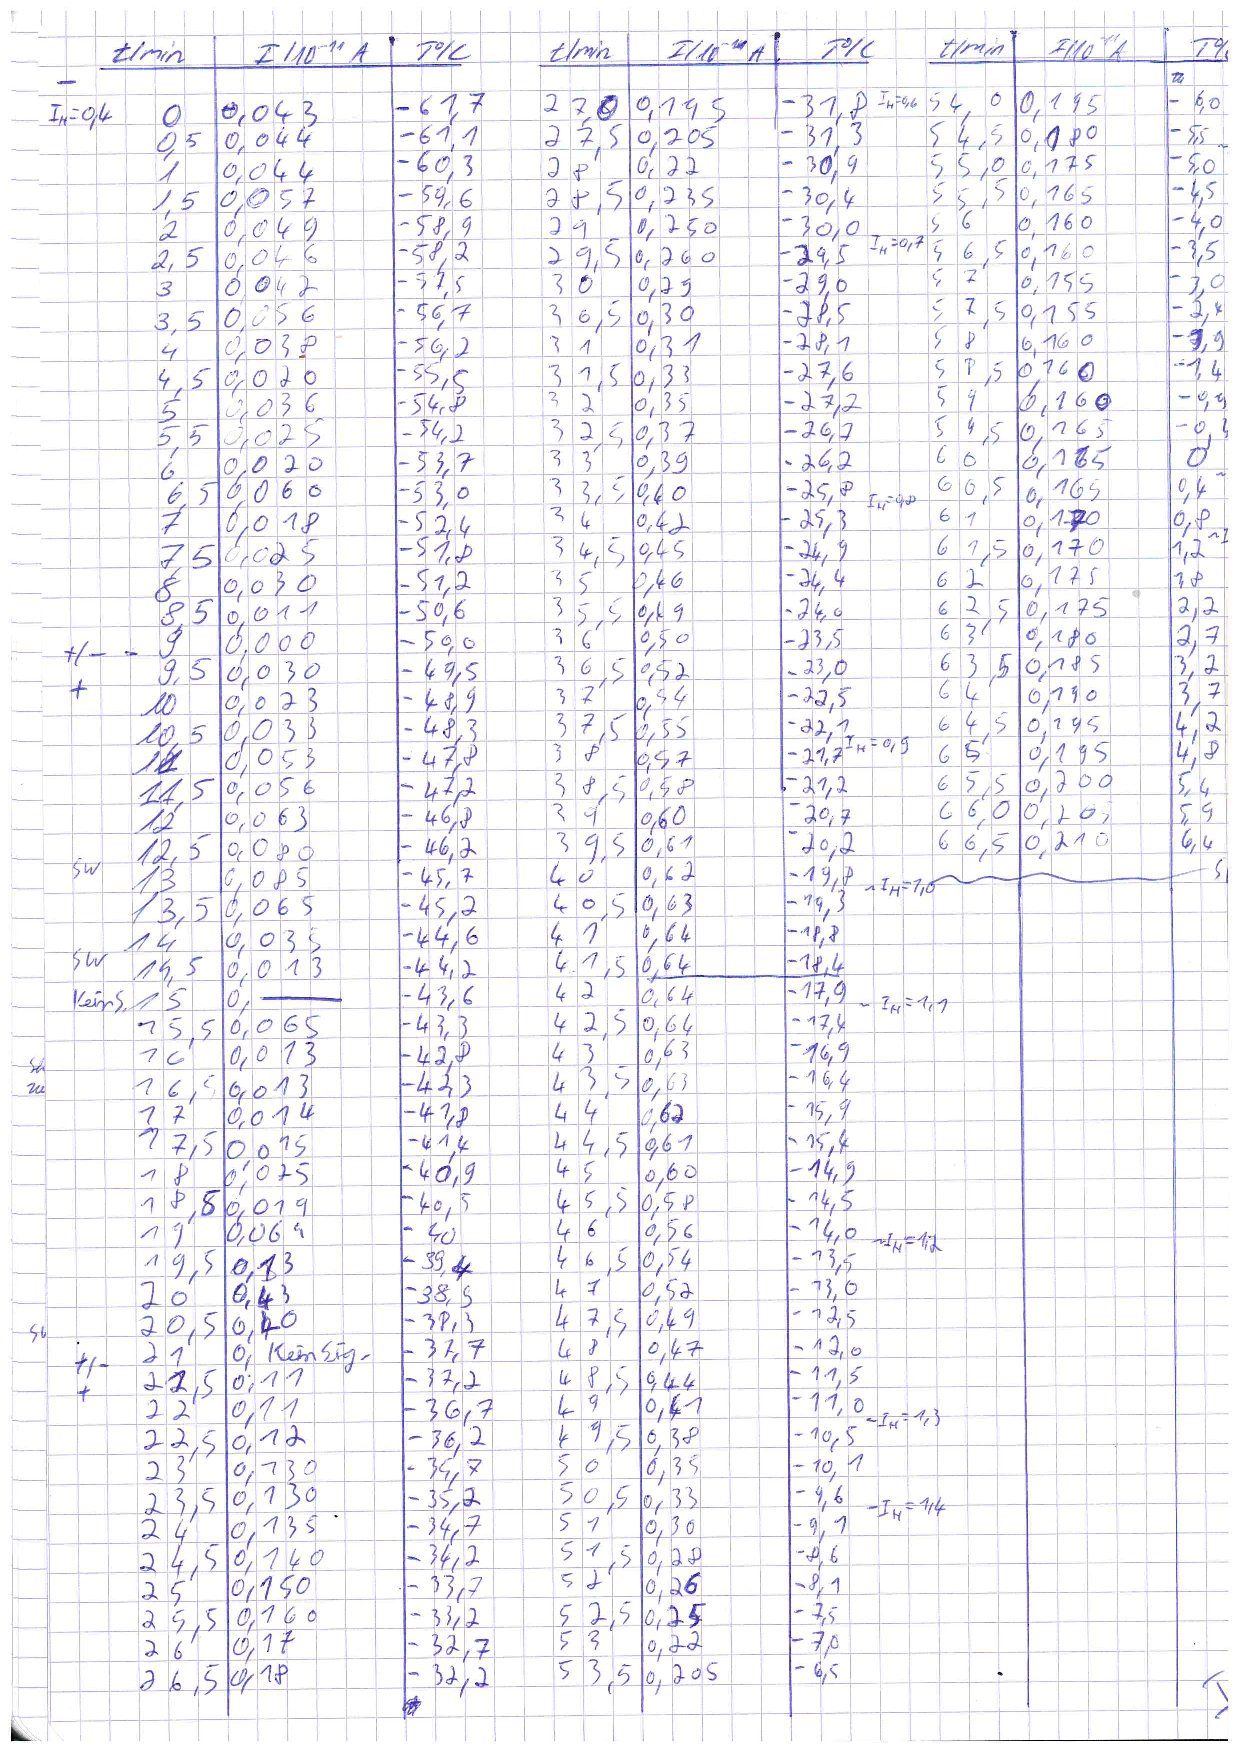
\includegraphics[height=\textheight]{data/Messdaten3.pdf}
\end{figure}

\end{document}
